\setcounter{page}{2}

\section{Задача}
Разглеждаме задачата за идеален топлинен контакт:
\begin{align}
	\frac{\partial u_1}{\partial t} & = \kappa_{1}  \frac{\partial ^ 2 u_1}{\partial x ^ 2}, - \infty < x < 0; 0 < t \leq T \\ 
	\frac{\partial u_2}{\partial t} & = \kappa_{2}  \frac{\partial ^ 2 u_2}{\partial x ^ 2}, 0 < x < \infty; 0 < t \leq T   
\end{align}
Където:
\begin{equation}
	\kappa_{i} = \frac{k_{i}}{\rho_{i} c_{i}}
\end{equation}

\begin{itemize}
	\item $\kappa_{i}$ - температуропроводност
	\item $k_{i}$ - топлопроводност
	\item $c_{i}$ - топлинен капацитет
	\item $\rho_{i}$  - плътност на материала
\end{itemize}

Наложено е следното прекъснато начално условие:
\begin{align}
	u_{1}(x, t = 0) & = 0, -\infty < x < 0  \\
	u_{2}(x, t = 0) & = u_0, 0 0 < x < \infty 
\end{align}

Както и гранични условия ,,на безкрайност``:
\begin{align}
	u_{1}(-\infty, t) & = 0, t > 0   \\
	u_{2}(+\infty, t) & = u_0, t > 0 
\end{align}
 
И условията за идеален контакт:
\begin{align}
	u_{1}(0, t)                                 & = u_2(0, t),  t > 0                                  \\
	k_{1}\frac{\partial u_1}{\partial x} (0, t) & = k_{2}\frac{\partial u_2}{\partial x} (0, t), t > 0 
\end{align}

Дефинираме ,,помощна константа`` $\beta$ с цел олекотяване на записа:
\begin{equation*}
	\beta = \frac{\sqrt{k_2 \rho_2 c_2}}{\sqrt{k_1 \rho_1 c_1}}
\end{equation*}

За така поставената задача е известно точното (аналитично решение):
\begin{align}
	u_{1}(x, t) & = \frac{\beta u_0}{1+\beta} \left[1 + \erf{\left(\frac{2}{2\sqrt{\kappa_1 t}}\right)}\right] \\
	u_{2}(x, t) & = \frac{u_0}{1+\beta} \left[\beta + \erf{\left(\frac{2}{2\sqrt{\kappa_2 t}}\right)}\right]   
\end{align}
Където: 
\begin{equation*}
	\erf{(z)} = \frac{2}{\sqrt{\pi}} \displaystyle\int_{0}^{z} e ^{-t^2} dt
\end{equation*}
За целите на изследването на полученото числено решение ще използваме следните физични пареметри за различни материали:\\
\begin{figure}[h]
	\centering
	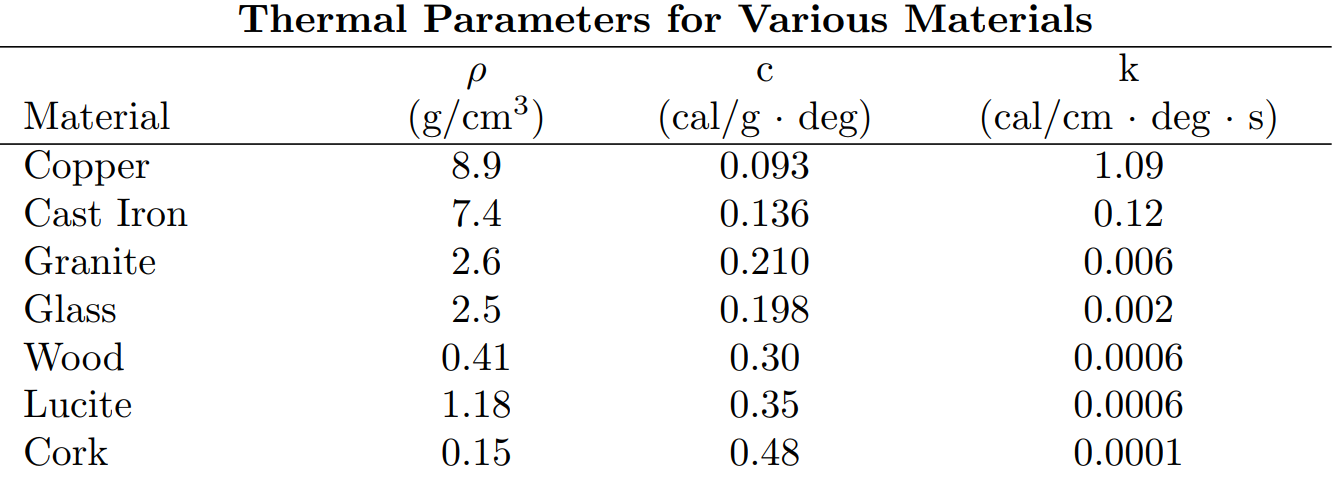
\includegraphics[width=\linewidth]{constants.png}
	\caption{Термофизични константи за различни материали}
	\label{fig:constants}
\end{figure}
